\setAuthor{Tundmatu autor}
\setRound{lahtine}
\setYear{2004}
\setNumber{G 3}
\setDifficulty{3}
\setTopic{Geomeetriline optika}

\prob{Taskulamp}
Taskulamp valgustab veekogu tasast põhja vee pinnaga risti suunatud paralleelse valgusvihuga. Kui valgusvihu teel kaugusele $H = \SI{120}{cm}$ veekogu põhjast paigutada lääts optilise tugevusega $D = \SI{2}{dptr}$ (lääts asub vee kohal nii, et läätse tasand on vee pinnaga paralleelne), siis põhja valgustatud ala pindala ei muutu. Leia veetaseme kõrgus antud veekogus. Vee murdumisnäitaja on $n = \num{1,33}$. On teada, et valgusvihu diameeter on palju väiksem läätse fookuskaugusest.

\emph{Vihje.} Väikeste nurkade puhul kehtib ligikaudne võrdus $\sin \alpha \approx \tan \alpha$.

\hint
Selleks, et põhja valgustatud ala pindala ei muutuks, peab äärmine kiir kalduma valgusvihi diameetri võrra horisontaalses suunas kõrvale. Kõrvalekaldumise määr on kõige mugavam arvutatav kasutades väikeste nurkade lähendust ning jaotades kõrvalekalde kaheks osaks; enne ja pärast vette sisenemist.

\solu

Läätse fookuskaugus on $f=1 / D=\SI{50}{cm}$. Et põhja valgustatud ala pindala ei muutuks, peab äärmine kiir kalduma $2 r$ võra horisontaalses suunas, kus $2 r$ on valgusvihu diameeter. Paralleelne valgusvihk peab läätse läbimisel koonduma fookuses, seetõttu äärmise kiire langemisnurk $\sin \alpha \approx \tan \alpha=r / f$. Siin me arvestasime, et $f \gg 2 r$. Murdumisseadusest $\sin \alpha=n \sin \beta$, kust $\tan \beta \approx \sin \beta=r / n f$. Kiire horisontaalses suunas
kaldumise tingimuse võime täisnurksetest kolmnurkadest lähtudes kirja panna kui
$$
(H-h) \tan \alpha+h \tan \beta=2 r.
$$
Asendades siia $\tan \alpha$ ja $\tan \beta$ väärtused ning avaldades $h$, saame
$$
h=\frac{H-2 f}{n-1}=\SI{80}{cm}.
$$
\begin{center}
	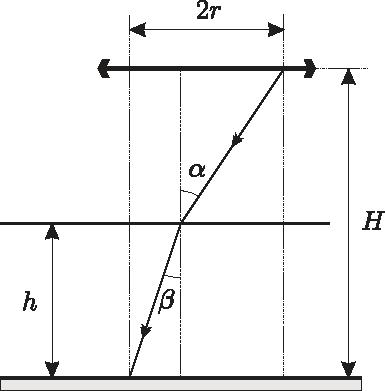
\includegraphics[width=0.5\linewidth]{2004-lahg-03-lah.pdf}
\end{center}
\probend